% +------------------------------------------------------------------------+
% | CGAL Reference Manual:  Subdivision_method_3
% +------------------------------------------------------------------------+
% | Subdivision surfaces on generic Polyhedron.
% | 
% | 1.2.2005  Le-Jeng Andy Shiue
% |
\RCSdef{\subdivisionRev}{$Id$}
\RCSdefDate{\subdivisionDate}{$Date$}
% +------------------------------------------------------------------------+

\newcommand\DS{Doo-Sabin}

% ------------------------------------------------------------------------
\newcommand\FIGDIR{Subdivision_method_3/FIG}
\newcommand\IL{{\itshape left}}
\newcommand\IR{{\itshape right}}
\newcommand\IM{{\itshape middle}}
\newcommand\IT{{\itshape top}}
\newcommand\IB{{\itshape bottom}}
% ------------------------------------------------------------------------

\ccParDims

\chapter{Subdivision Methods}
\label{chapterSubdivision}
\ccChapterRelease{\subdivisionRev. \ \subdivisionDate}
\ccChapterAuthor{Le-Jeng Andy Shiue}
\hspace{.4cm}
\begin{ccTexOnly}
    \setlength{\unitlength}{1mm}
    \begin{picture}(0,0)(0.0,0.0)
      \put (78,25){% textwidth = 156mm
          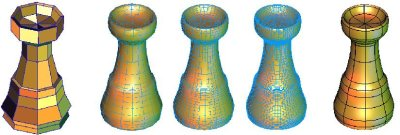
\includegraphics[width=0.45\textwidth]{\FIGDIR/QTSub}
      }
    \end{picture}\vspace{-4mm}% compensate for some vspace added by picture
\end{ccTexOnly}

\minitoc

% +------------------------------------------------------------------------+
\section{Introduction} \label{sectionSubIntro}
% +------------------------------------------------------------------------+
The subdivision method is a simple yet powerful way to 
generate smooth surfaces from arbitrary polyhedral meshes. 
Unlike spline-based surfaces (e.g NURBS) or other numeric-based 
modeling techniques, users of subdivision
surfaces do not need in-depth mathematics 
knowledge on subdivision methods. Users only need
natural geometric intuitions to control the subdivision 
surface; hence subdivision methods are popular choices for
character modeling in video games and character animations.

%Subdivision algorithms (see e.g.~\cite{cgal:ww-smgd-02})
%recursively refine coarse meshes and generate ever closer 
%approximations to a smooth surface.
%for character animation, surface modeling, or physics simulation.
%Setting aside the specific strategy of geometric averaging
%for the new points, subdivision algorithms can be classified 
%according to the topological refinement of the underlying mesh.
%\ccc{Subdivision_method_3}, working on the concept of the 
%\ccc{CGAL::Polyhedron_3} (see Chapter~\ref{chapterPolyhedron}),
%takes advantage of this separation of geometry and topology.
%Each subdivision algorithm is a refinement function parametrized
%by a set of rountines of geometric averageing.

\ccc{Subdivision_method_3} aims to be simple to use and extend.
It supports four most used subdivision methods, including Loop, 
Catmull-Clark, Doo-Sabin and $\sqrt{3}$ subdivisions. Variations 
of these methods can be easily implemented by plugging 
in the user-defined computation rules. \ccc{Subdivision_method_3}
is designed to work on \ccc{CGAL::Polyhedron_3} 
(see Chapter~\ref{chapterPolyhedron}), 


\begin{ccHtmlOnly}
     <CENTER>
         <img src="./FIG/QTSub.jpg" alt="QT subdivision on a rook model"><P>
     </CENTER>
\end{ccHtmlOnly}

% +------------------------------------------------------------------------+
\section{Subdivision Algorithms}
\label{secSubAlgo}
% +------------------------------------------------------------------------+
In this chapter, we explain some fundamentals of 
subdivision methods. We only focus on the topics helping you 
to understand the design of the package; interested readers can
still refer to \cite{cgal:ww-smgd-02} for an in-depth introduction.
Some terminologies introduced in this section will be used again
in later sections. If you are only interested in using a 
specific subdivision method, Section \ref{secFirstSub} 
gives a quick tutorial on Catmull-Clark subdivision.

A subdivision method recursively refines a coarse mesh and 
generates an ever closer approximation to a smooth surface.
The coarse mesh can have arbitrary shapes, but it has to 
be a 2-manifold. In a 2-manifold, every interior point has 
a neighborhood homomorphic to a 2D disk. Subdivision methods
on non-manifolds have be developed, but are not considered
in this work. 
%Subdivision algorithms (see e.g.~\cite{cgal:ww-smgd-02}) 
%define surfaces as the limit
%of recursive refinement of a polyhedral mesh, called
%\emph{control mesh}. 
%The refinements generate mesh points 
%to be smoothed to approximate the limit surface.   
The chapter teaser shows the process of a subdivision method on 
a chess model. The coarse chess is repeatly refined by a pattern, 
and more and more points are generated to approximate the 
smooth chess.

Many refinement patterns are used in practice. 
\ccc{Subdivision_method_3} supports the four most popular 
patterns, and each of them is used by 
Catmull-Clark\cite{cgal:cc-rgbss-78}, Loop, Doo-Sabin 
and $\sqrt{3}$ subdivision (left to right in the 
figure). Note we name these patterns by their topological
characteristics, not the associated subdivision methods. 
PQQ indicates the \emph{P}rimal \emph{Q}uadtrateral \emph{Q}uadrisection. 
PTQ indicates the \emph{P}rimal \emph{T}riangle \emph{Q}uadrisection. 
DQQ indicates the \emph{D}ual \emph{Q}uadtrateral \emph{Q}uadrisection.
$\sqrt{3}$ has a long story of its naming; simply put, it 
indicates the speed of the topological converging.

\begin{ccTexOnly}
  \begin{center}
    \parbox{0.6\textwidth}{%
      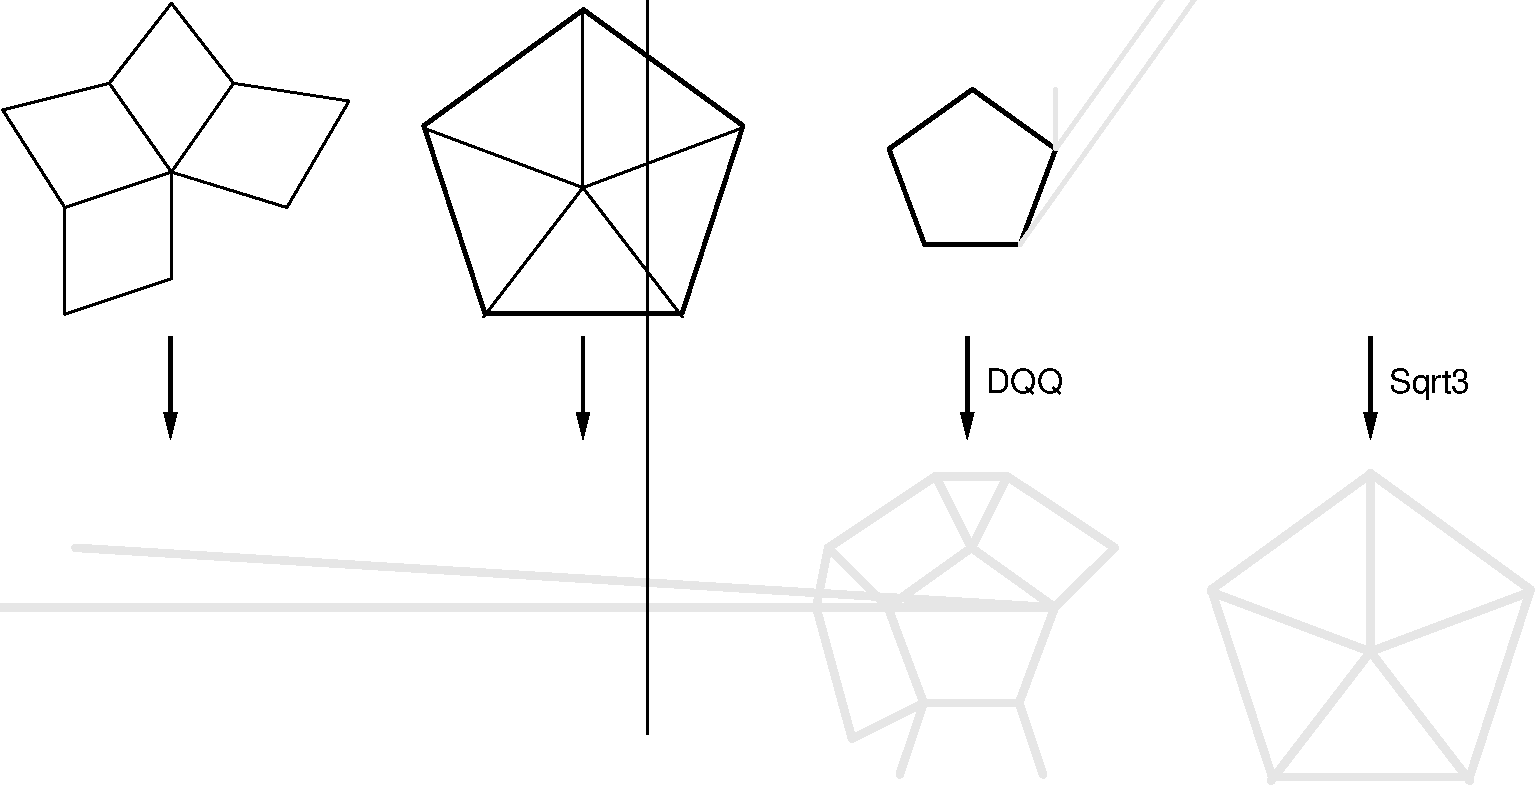
\includegraphics[width=0.6\textwidth]{\FIGDIR/RefSchemes}%
    }\\ \vspace{0.5cm}
  \end{center}
\end{ccTexOnly}

\begin{ccHtmlOnly}
  <CENTER>
     <img src="./FIG/RefSchemes.gif" alt="Refinement Hosts"><P>
  </CENTER>
\end{ccHtmlOnly}

The figure demonstrates these four refinement patterns on 
the 1-disk of a valence-5 vertex/facet.
Refined meshes are shown below the source meshes. 
%We call a source mesh \emph{control mesh} if it is
%the origin of a squence of refinements.
Points on the refined mesh are generated by averaging
neighbor points on the source mesh. A graph, called \emph{stencil}, 
determines the source neighthood whose points contribute to the 
position of a refined point. A refinement pattern usually has 
several specific sets of stencils.
%Stencils are defined at the time the refinement pattern is chosen.  
%as illustrated in Figure \ref{fig:RefMap},
For example, the PQQ
%\emph{P}rimal \emph{Q}uadtrateral \emph{Q}uadrisection (PQQ) scheme 
refinement used by Catmull-Clark subdivision has a vertex-node stencil, 
which defines the 1-ring of an input vertex; an edge-node stencil, 
which defines the 1-ring of an input edge; and a facet-node stencil, 
which defines an input facet. The stecils of the PQQ refinement are
shown in the following figure. The blue neighborhoods in the 
top row indicate the corresponding stencils of the refined nodes 
in red. 

\begin{ccTexOnly}
  \begin{center}
    \parbox{0.5\textwidth}{%
      
\includegraphics[width=0.5\textwidth]{\FIGDIR/PQQStencil}%
    }\\ \vspace{0.5cm}
  \end{center}
\end{ccTexOnly}

\begin{ccHtmlOnly}
  <CENTER>
     <img src="./FIG/PQQStencil.gif" alt="Stencils of PQQ scheme "><P>
  </CENTER>
\end{ccHtmlOnly}


%while the DQQ scheme has only a corner-node stencil, which 
%relates the facet of a corner to a target node.
Stencils with weights are called \emph{geometry masks}.
%One practical set of geometry masks of the PQQ scheme is
A subdivision method defines the masks for the stencils, and 
generates new points by summarizing source points weighted by the mask. 
Geometry masks are usually carefully choosed to meet requirements of 
certain surface smoothness and shape quality.
The geometry masks of Catmull-Clark subdivision are shown
below (masks for extraordinary vertices are not shown).  

\begin{ccTexOnly}
  \begin{center}
    \parbox{0.4\textwidth}{%
      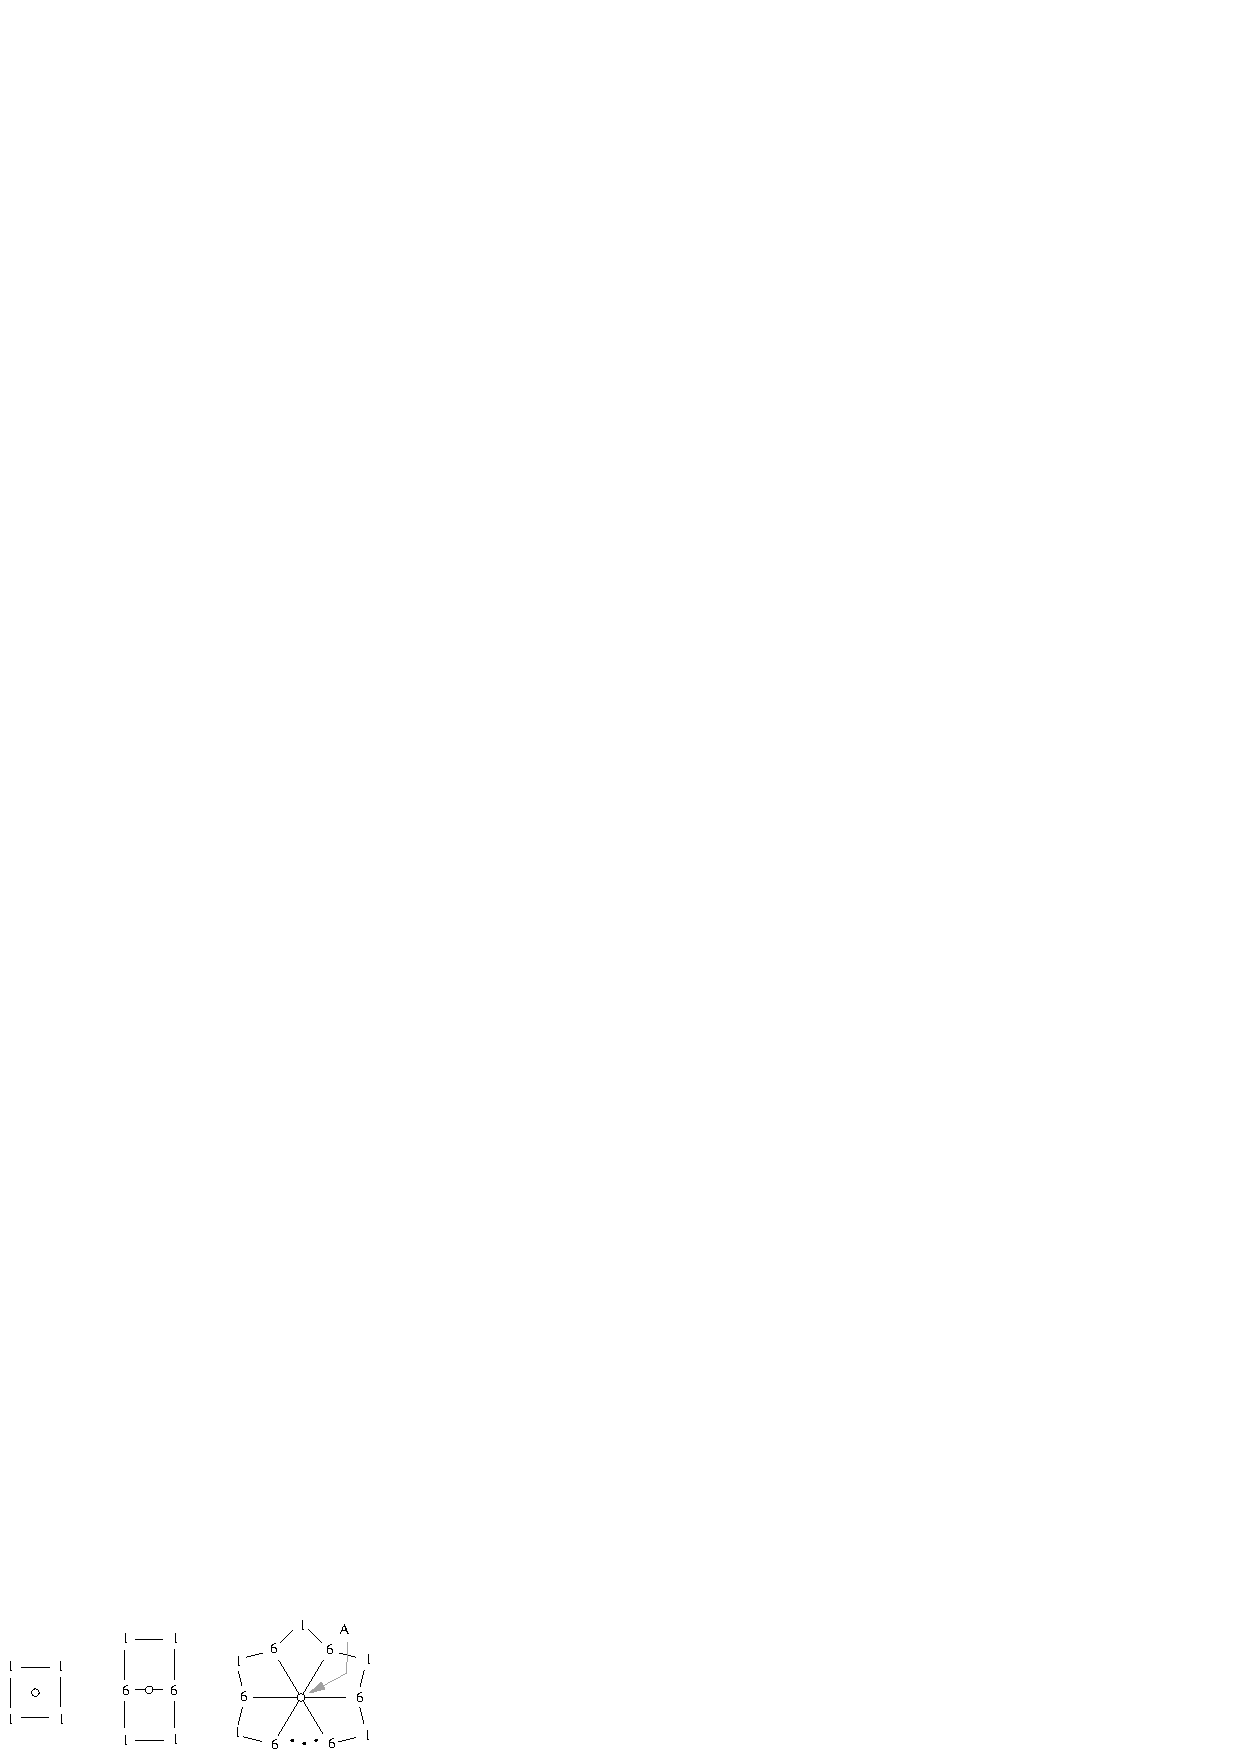
\includegraphics[width=0.4\textwidth]{\FIGDIR/cc_mask}%
    } \\ \vspace{0.5cm}
  \end{center}
\end{ccTexOnly}

\begin{ccHtmlOnly}
  <CENTER>
     <img src="./FIG/cc_mask.gif" alt="Catmull-Clark geometry stencil"><P>
  </CENTER>
\end{ccHtmlOnly}

The weights shown here are unnormalized, and $n$ is the valence 
of the vertex. The generated point, in red, is computed by a summation
of the weighted points. For example, a Catmull-Clark facet-node is 
computed by the summation of $1/4$ of each points on its stencil.

A stencil may have several specific sets of geometry masks. In other 
words, a facet-node of Catmull-Clark refinement may be computed by 
the summation of $1/5$ of each stencil node instead of $1/4$. 
Although it is legal in \ccc{Subdivision_method_3} to have 
any kind of geometry mask, the result surfaces may be odd, 
not smooth, or not even exist. \cite{cgal:ww-smgd-02} explains the 
details on designing masks of quality subdivision surfaces.

%The averaging process can typically be factored into 
%simpler steps \cite{Oswald-2003-CSS}.
%and this has been implemented in the OpenMesh library \cite{Sovakar-2004-APISUB}.
%However, while stencil factoring simplifies the implementation,
%it is less efficient because it requires repeated visits 
%to all nodes.

%% Since only a fixed number of refinement patterns are 
%% practical but a wide variety of geometry masks can be developed,
%% \ccc{Subdivision_method_3} provides a set of refinement patterns 
%% (the \emph{refinement hosts})
%% and hands the definition of geometry masks
%% (the \emph{geometry policies}) to the library user.
%% A subdivision scheme is obtained by parameterizing the 
%% refinement host with geometry policies. 
%% For example, Catmull-Clark subdivision is constructed by 
%% parameterizing the PQQ refinement with the Catmull-Clark geometry 
%% policies.

%, which compute the smoothed points based on the
%Catmull-Clark geometry masks.

%A subdivision scheme of \ccc{CGAL::Subdivision_method_3} is a 
%refinement host parameterized with a geometry policy. 

%The refinement host realizes the topological refinement and 
%the stencils. The geometry policy consists a set of 
%averaging rules of the geometry stencils.

% +-------------------------------------------------------------+
\section{Create Your First Subdivision Surafce}
\label{secFirstSub}
Assuming your familiarity of \ccc{CGAL::Polyhedron_3},
you can intergrate \ccc{Subdivision_method_3} into your program 
without much effort.

\ccIncludeExampleCode{Subdivision_method_3/CatmullClark_subdivision.C}

This example demonstrates the use of Catmull-Clark subdivision
on a CGAL polyhedron. The polyhedron is restricted within the Cartesian
space, where most subdivision applications are designed to work.
There is only one line deserving a detailed explanation:
\begin{ccExampleCode}
Subdivision_method_3::CatmullClark_subdivision(P,d);
\end{ccExampleCode}
\ccc{Subdivision_method_3} specifies the namespace of our
subdivision functions. \ccc{CatmullClark_subdivision(P,d)} computes the 
Catmull-Clark subdivision surfaces of the polyhedron \ccc{P} after
\ccc{d} iterations of the refinements. The polyhedron \ccc{P} is 
passed by the reference and is modified (i.e.~subdivided) by the 
subdivision function.

Other subdivision methods (such as Doo-Sabin subdivision) can be
used with the same level of the ease.

This example shows how to subdivide a simple \ccc{CGAL::Polyhedron_3}
with \ccc{Subdivision_method_3}.
An application-defined polyhedron might use a specialized kernel and/or
a specialized internal container. There are two major restrictions on the 
your application-defined polyhedron to be able to work with 
\ccc{Subdivision_method_3}.
\begin{itemize}
\item
\ccc{Point_3} is type-defined within the kernel. Without \ccc{Point_3} 
and associated operations being defined, \ccc{Subdivision_method_3} 
can not know how to compute and where to store the new vertex points.
\item
The primitives (such as vertices, halfedges and facets) 
in the internal container are sequentially ordered. 
In other words, the iterators traverse the primitives in 
the order of their creation. Examples include \ccc{std::vector} and 
\ccc{std::list}.

\end{itemize}

Section~\ref{secRefHost} gives detailed explanations on these 
two restrictions.

% +-------------------------------------------------------------+
\section{Catmull-Clark Subdivision in Depth}
\label{secCC}
%Loop, Catmull-Clark, Doo-Sabin and $\sqrt{3}$ subdivision methods
%are popular in practice. Yet from time to time you may want to
%create your own method. You may be a graduate student believing 
%in a perfect subdivision scheme, or
%you just want a unique surface which looks simply bad. In either case,
%\ccc{Subdivision_method_3} allows you to try your beloved algorithms
%with a small amount of efforts. The best way to learn how to create
%a your-name subdivision is by digging into one of the four subdivisions
%\ccc{Subdivision_method_3} supported. 
%In this section, we will guide you through the implementation of 
%Catmull-Clark subdivision.
%This section explain how do we implement the
%Catmull-Clark subdivision based on the framework of 
%\ccc{Subdivision_method_3}.
\ccc{Subdivision_method_3} gives you easy-to-use functions on 
Catmull-Clark, Loop, Doo-Sabin and $\sqrt{3}$ subdivision methods.
But \ccc{Subdivision_method_3} is more like a framework that let 
you extend the methods with ease. This section explains the process
of \emph{implementing} the Catmull-Clark subdivision within
\ccc{Subdivision_method_3}. Following this procedure, you can 
easily implement a new subdivision method based on the refinement 
patterns in \ccc{Subdivision_method_3}

When a subdivision method is developed, a refinement pattern is 
chosen, and then a set of geometry masks are developed to 
\emph{position} the new points.
E. Catmull and J. Clark picked the \emph{P}rimal \emph{Q}uadtrateral 
\emph{Q}uadrisection (PQQ) to be the refinement pattern,
and developed a set of geometry masks to generate (or more precisely, 
to approximate) the B-spline surface from the control polyhedral 
mesh. 

There are three key components of implementing
Catmull-Clark subdivision: 
\begin{itemize}
\item
a mesh data structure that can represent arbitrary 2-manifolds, 
\item
a process that refines the mesh data structure, 
\item
and the geometry masks that compute and assign the new points.
\end{itemize}

%We have the mesh data structure in \ccc{CGAL::Polyhedron_3}, and 
%we have the PQQ refinement in \ccc{Subdivision_method_3} that 
%works on \ccc{CGAL::Polyhedron_3}. But we still need the 
%geometry masks to finish the job.
%\ccc{Subdivision_method_3} also supports three other refinements that 
%you can choose to use for your subdivision. These refinements are
%PT(riangle)Q for Loop subdivision, D(ual)QQ for Doo-Sabin subdivision, 
%and $\sqrt{3}$ triangulation for $\sqrt{3}$ 
%subdivision. Here is the function declaration of the PQQ refinement.
\ccc{Subdivision_method_3} defines a function that covers all 
three components for Catmull-Clark subdivision.

\begin{ccExampleCode}
template <class Polyhedron, template <typename> class Mask>
void PQQ(Polyhedron& p, Mask<Polyhedron> mask, int depth)
\end{ccExampleCode}

\ccc{Polyhedron} is a model of \ccc{CGAL::Polyhedron_3}, which
is a mesh data structure that can represent arbitrary 
2-manifolds. \ccc{PQQ(...)} provides the process refining 
the control polyhedron \ccc{p}. During the refinement, 
\ccc{PQQ(...)}, the \emph{refinement host}, computes and assigns the 
new points by communicating with the \ccc{mask}. 
To implement Catmull-Clark subdivision,
\ccc{Mask}, the \emph{geometry policy}, has to realize the geometry 
masks of Catmull-Clark subdivision. 
\ccc{depth} specifies how many steps of the refinement 
to be applied on the polyhedron. 
%To make the call to
%\ccc{PQQ} a Catmull-Clark subdivision, the only thing left is to
%implement a geometry policy realizing the Catmull-Clark geometry masks.

To implement the geometry masks, we need to know how  
a mask communicates with the refinement host. The PQQ refinement 
defines three stencils, and therefor three geometry masks
are required for Catmull-Clark subdivision.
The interfaces of the stencils are specified like 
the policy class \ccc{PQQ_stencil_3}.

\begin{ccExampleCode}
template <class Polyhedron>
class PQQ_stencil_3 {
  void facet_node(Facet_handle facet, Point& pt);
  void edge_node(Halfedge_handle edge, Point& pt);
  void vertex_node(Vertex_handle vertex, Point& pt);
};
\end{ccExampleCode}

Now we can compute the new points using the primitive handle
passed into the policy functions, and assign the result to
\ccc{Point& pt}. Since our goal is to implement Catmull-Clark 
subdivision, we need to implement the policy functions by its 
geometry masks. 
%For clarity, we rename the policy class 
%to indicate geometry masks are in place.

\begin{ccExampleCode}
template <class Polyhedron>
class CatmullClark_mask_3 {
  void facet_node(Facet_handle facet, Point& pt) {
    Halfedge_around_facet_circulator hcir = facet->facet_begin();
    int n = 0;
    FT p[] = {0,0,0};
    do {
      Point t = hcir->vertex()->point();
      p[0] += t[0], p[1] += t[1], p[2] += t[2]; 
      ++n;
    } while (++hcir != facet->facet_begin());
    pt = Point(p[0]/n, p[1]/n, p[2]/n);
  }
  void edge_node(Halfedge_handle edge, Point& pt) {
    Point p1 = edge->vertex()->point();
    Point p2 = edge->opposite()->vertex()->point();
    Point f1, f2;
    facet_node(edge->facet(), f1);
    facet_node(edge->opposite()->facet(), f2);
    pt = Point((p1[0]+p2[0]+f1[0]+f2[0])/4,
               (p1[1]+p2[1]+f1[1]+f2[1])/4,
               (p1[2]+p2[2]+f1[2]+f2[2])/4 );
  }
  void vertex_node(Vertex_handle vertex, Point& pt) {
    Halfedge_around_vertex_circulator vcir = vertex->vertex_begin();
    int n = circulator_size(vcir);    

    float Q[] = {0.0, 0.0, 0.0}, R[] = {0.0, 0.0, 0.0};
    Point& S = vertex->point();
    
    Point q;
    for (int i = 0; i < n; i++, ++vcir) {
      Point& p2 = vcir->opposite()->vertex()->point();
      R[0] += (S[0]+p2[0])/2;
      R[1] += (S[1]+p2[1])/2;
      R[2] += (S[2]+p2[2])/2;
      facet_node(vcir->facet(), q);
      Q[0] += q[0];      
      Q[1] += q[1];      
      Q[2] += q[2];
    }
    R[0] /= n;    R[1] /= n;    R[2] /= n;
    Q[0] /= n;    Q[1] /= n;    Q[2] /= n;
      
    pt = Point((Q[0] + 2*R[0] + S[0]*(n-3))/n,
               (Q[1] + 2*R[1] + S[1]*(n-3))/n,
               (Q[2] + 2*R[2] + S[2]*(n-3))/n );
  }
};
\end{ccExampleCode}

Note types used in this example (such as \ccc{Point} and
\ccc{Facet_handle}) are assumed to be type-defined within the
\ccc{Polyhedron}. This \ccc{CatmullClark_mask_3} is designed
to work on a \ccc{CGAL::Polyhedron_3} with the default CGAL 
kernel geometry. You may need to rewrite the geometry computation
in the code to match the kernel geometry of your application.

To excute the subdivision, you can 
simply call the \ccc{PQQ(...)} with the Catmull-Clark mask
we just designed.

\begin{ccExampleCode}
PQQ(p, CatmullClark_mask_3<Polyhedron>(), depth);
\end{ccExampleCode}

%\begin{ccExampleCode}
%template <class Polyhedron>
%void CatmullClark_subdivision(Polyhedron& p, int depth) {
%    PQQ(p, CatmullClark_mask_3<Polyhedron>(), depth);
%}
%\end{ccExampleCode}

Loop, Doo-Sabin and $\sqrt{3}$ subdivisions are implemented 
with a similar process: pick a refinement host and implement 
the geometry policy. To develop your own subdivision with 
\ccc{Subdivision_method_3}, the key is 
to find the right combination of the host and the policy, 
which are explained in the following sections.

% +-------------------------------------------------------------+
\section{Refinement Host}
\label{secRefHost}
\ccc{Subdivision_method_3} provides four refinement hosts of primal 
quadrilateral quadrisection (PQQ), primal triangle 
quadrisection (PTQ), dual quadrilateral 
quadrisection (DQQ) and $\sqrt{3}$ triangulation, which 
are used by Catmull-Clark, Loop, \DS\ and $\sqrt{3}$ subdivision, 
respectively. 

\begin{ccTexOnly}
  \begin{center}
    \parbox{0.6\textwidth}{%
      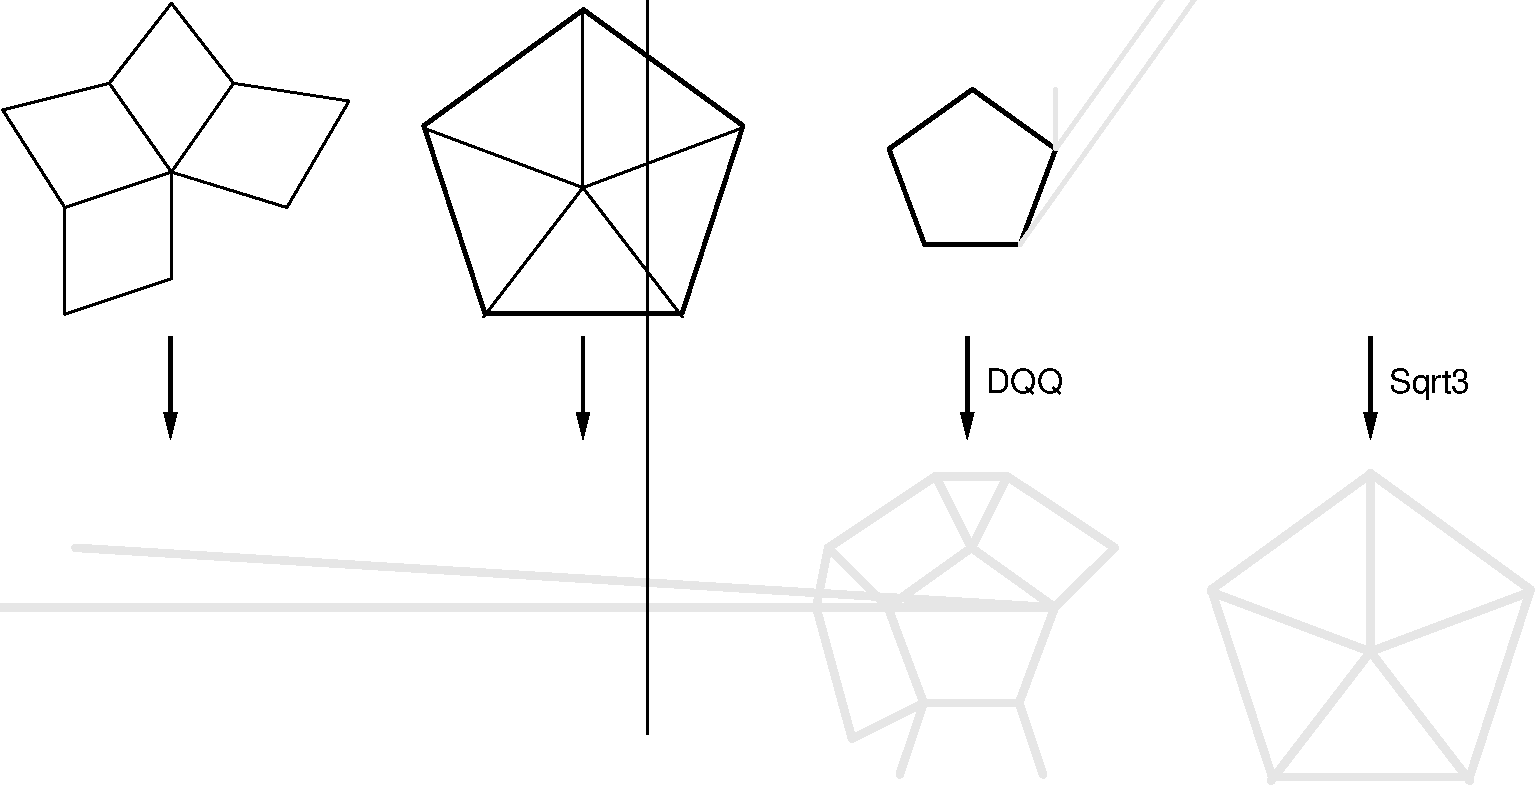
\includegraphics[width=0.6\textwidth]{\FIGDIR/RefSchemes}%
    }\\ \vspace{0.5cm}
%    \ccc{Subdivision_method_3} supports hosts of these four refinement 
%    schemes that are demonstrated on a valence-n submesh.
%    The refined mesh is shown below the control mesh.
  \end{center}
\end{ccTexOnly}

\begin{ccHtmlOnly}
  <CENTER>
     <img src="./FIG/RefSchemes.gif" alt="Refinement Hosts"><P>
  </CENTER>
\end{ccHtmlOnly}


\begin{ccExampleCode}
template <class Polyhedron>
class Subdivision_method_3 {
  // S is the geometry policy realizing the geometry masks
  template <template <typename> class S>
  static void PQQ(Polyhedron& p, S<Polyhedron> rule, int step);

  template <template <typename> class S>
  static void PTQ(Polyhedron& p, S<Polyhedron> rule, int step);

  template <template <typename> class S>
  static void DQQ(Polyhedron& p, S<Polyhedron> rule, int step);

  template <template <typename> class S>
  static void Sqrt3(Polyhedron& p, S<Polyhedron> rule, int step);
}
\end{ccExampleCode}

%% Stencils are maintained using the iteration concept
%% to avoid the need for vertex tags to distinguish
%% the stencil types.
%% For example, on a PQQ refined mesh, the vertex iterator 
%% visits the 
%% vertex-nodes, edge-nodes and then facet-nodes. The visit
%% order is implicitly used to determine the stencil of
%% the visited node.

Each refinement host is a template function of
a polyhedron type and a policy type. The polyhedron type is
a model of the \ccc{CGAL::Polyhedron_3} concept, and the
policy type is a class with functions realizing the 
geometry masks of a specific subdivision scheme.

Refinement hosts refine the polyhedron, maintain the stencils 
(i.e.~the mapping between the control mesh and the refined mesh), 
and call policy functions to compute and assign the new points. 
In our implementation, refinements are done by applying a 
sequence of connectivity operations (mostly Euler operations).
The stencils are maintained by ordering nodes on the refined 
polyhedron to match the sequence of the connectivity operations. 
By matching the order, no flag to classify the stencils 
is required to maintain and access the stencils.
But to make the ordering trick work, the polyhedron type need 
to use an internal storage with sequential ordering, such as
a vector or a linked-list. A sequential ordered container inserts
new entries at the end, and its iterator visits the entries in the 
order of their insertion. Non-sequential structures such as 
tree or map do not provide the required ordering, and hence
can not be used with \ccc{Subdivision_method_3}.
 
Although \ccc{Subdivision_method_3} does not require flags or 
tags to support the refinements and the stencil accesses, it
still need to know how to compute and where to store the geometry
data (in most cases, the points). \ccc{Subdivision_method_3} 
expects that the typename \ccc{Point_3} is 
defined in the scope of \ccc{Polyhedron} and \ccc{Polyhedron::Vertex}. 
The refinement hosts use
this point type as the geometry holder and delegate the geometry
computation to the geometry policies. The geometry policy is 
explained in next section. 

For details of the refinement algorithm and implementation, 
interested users can refer to \cite{cgal:sp-mrbee-05}.

% +-------------------------------------------------------------+
\section{Geometry Policy}
A geometry policy defines a set of geometry masks. 
Each geometry mask is realized as a member function (i.e.~the 
policy function) computing and assigning new points according 
to a particular subdivision scheme. 
%The policy interface is defined with the refinement host. 

Each policy function receives a primitive handle 
(e.g.~\ccc{Halfedge_handle}) of the control polyhedron, 
and the reference of the \ccc{Point} to the refined vertex. 
In general, the implementation of the policy function 
collects the neighbors of the primitive handle (i.e.~nodes 
on the stencil), and (ideally) computes the new point 
by a linear combination of the stencil 
nodes and the mask (i.e.~the stencil weights).

\begin{ccTexOnly}
  \begin{center}
    \parbox{0.4\textwidth}{%
      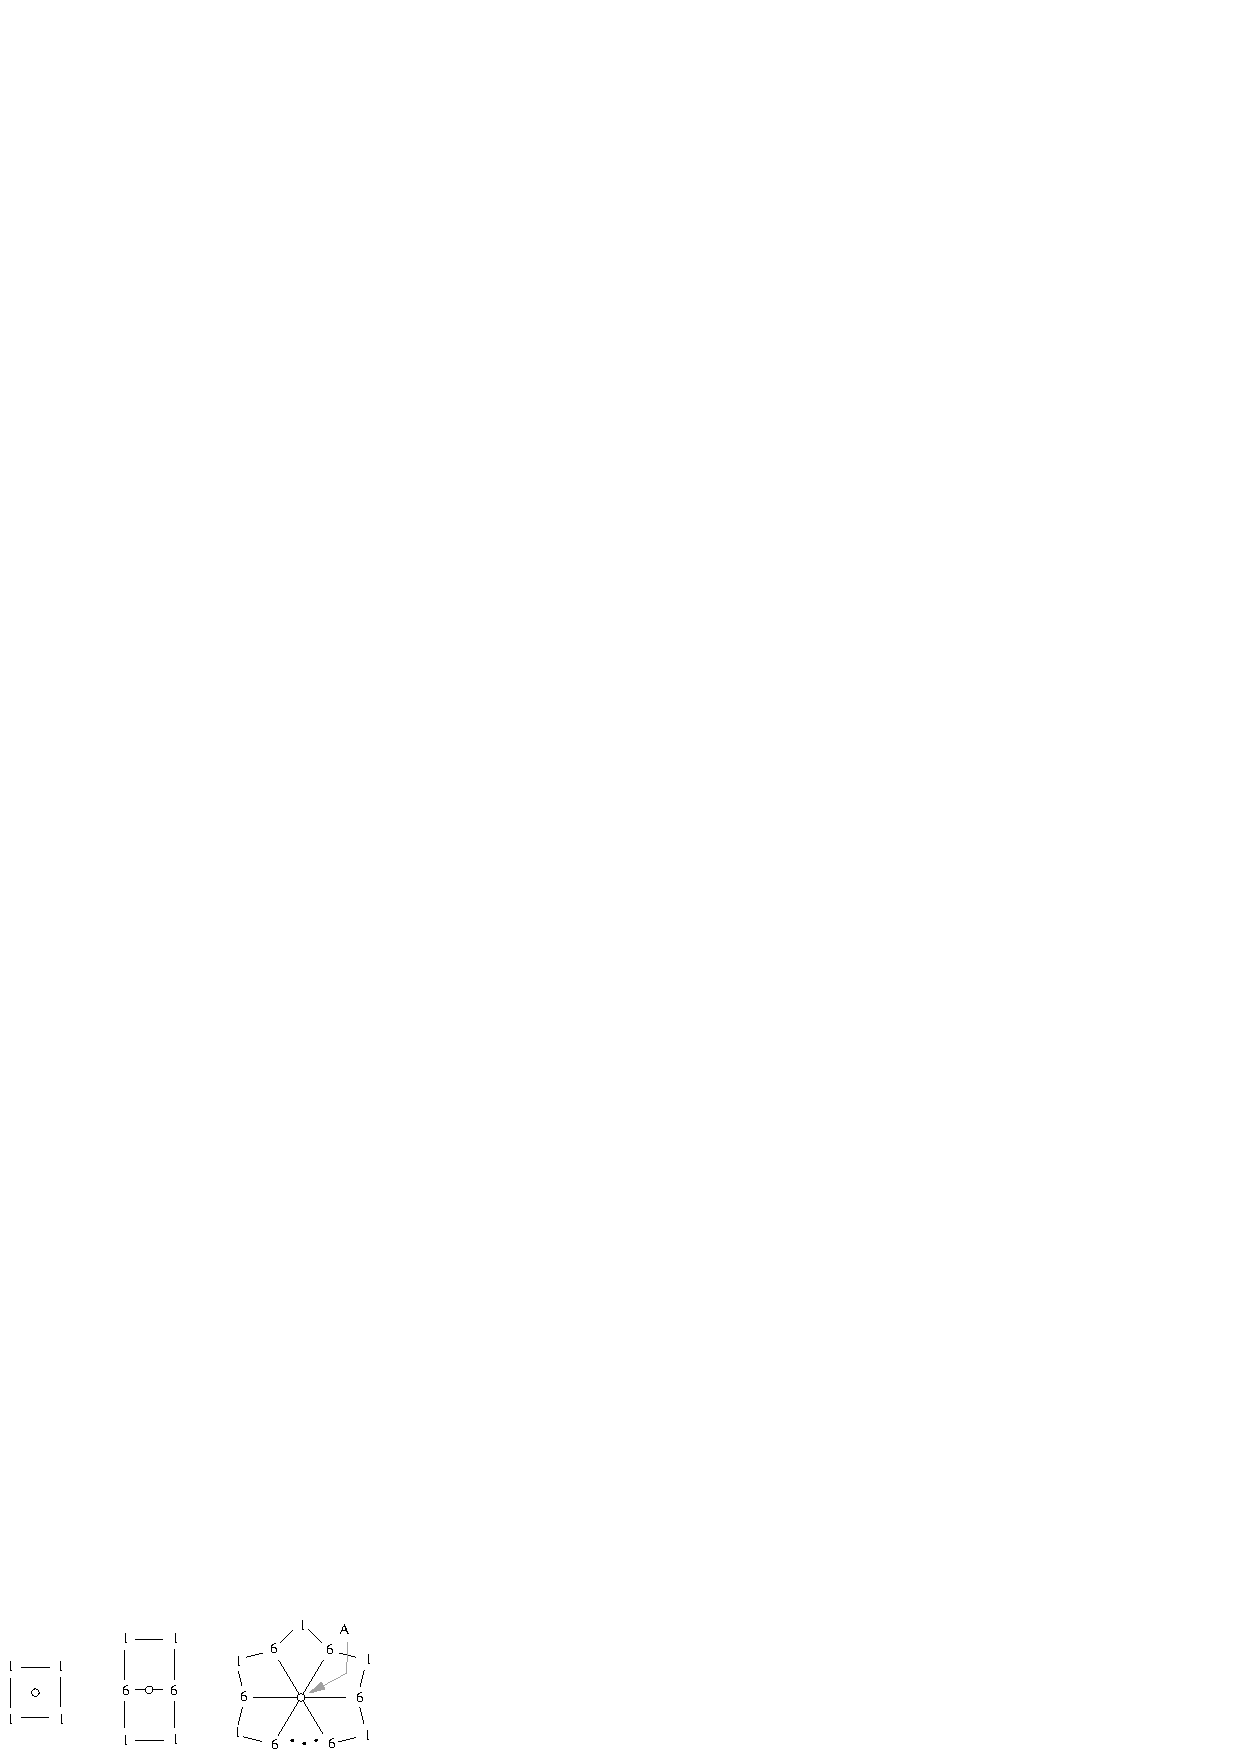
\includegraphics[width=0.4\textwidth]{\FIGDIR/cc_mask}%
    } \\ \vspace{0.5cm}
  \end{center}
\end{ccTexOnly}
\begin{ccHtmlOnly}
  <CENTER>
     <img src="./FIG/cc_mask.gif" alt="Catmull-Clark geometry stencil"><P>
  </CENTER>
\end{ccHtmlOnly}

This picture shows the stencils and the geometry masks for
Catmull-Clark subdivision. The weights shown here are unnormalized, 
and $n$ is the valence of the vertex. The new points are 
computed by the summation of the weighted points on their stencils.
Following codes show an implementation of the geometry policy of 
the facet-node. \ccc{Point} is a typedef to the \ccc{Point_3}
in \ccc{Polyhedron}. Note when \ccc{n} is $4$, this policy computes 
the facet-node shown in the above picture. The complete listing
of the Catmull-Clark policy class is in the Section~\ref{secCC}.

\begin{ccExampleCode}
template <class Polyhedron>
class CatmullClark_mask_3 {
  void facet_node(Facet_handle facet, Point& pt) {
    Halfedge_around_facet_circulator hcir = facet->facet_begin();
    int n = 0;
    FT p[] = {0,0,0};
    do {
      Point t = hcir->vertex()->point();
      p[0] += t[0], p[1] += t[1], p[2] += t[2]; 
      ++n;
    } while (++hcir != facet->facet_begin());
    pt = Point(p[0]/n, p[1]/n, p[2]/n);
  }
}
\end{ccExampleCode}

In this example, \ccc{Point} is assumed to be a \ccc{CGAL::Point_3}.
But you are allowed to use any point \emph{type} as long as it is type
defined as \ccc{Point_3} in your polyhedron class and vertex class.
You may need to modify the geometry policy to support the computation
and assignment of your specialized point. This extension is not unusual 
in graphics applications. For example, you might want to subdivide the
texture coordinates when you subdivide the polyhedron. The typename 
\ccc{Point_3} is actually the attribute holder, including the 
point of course, for the vertices.

The PQQ refinement host requires three policy functions for 
polyhedrons without open boundaries: a vertex-node 
stencil, an edge-node stencil, and a facet-node stencil. 
To support polyhedrons with boundaries, a policy function
for border vertices is also required. The border policy for
Catmull-Clark is given below.

%% \begin{ccTexOnly}
%%   \begin{center}
%%     \parbox{0.5\textwidth}{%
%%       
\includegraphics[width=0.5\textwidth]{\FIGDIR/PQQStencil}%
%%     }
%%   \end{center}
%% \end{ccTexOnly}

\begin{ccExampleCode}
  void border_node(Halfedge_handle edge, Point& ept, Point& vpt) {
    Point& ep1 = edge->vertex()->point();
    Point& ep2 = edge->opposite()->vertex()->point();
    ept = Point((ep1[0]+ep2[0])/2, (ep1[1]+ep2[1])/2, (ep1[2]+ep2[2])/2);

    Halfedge_around_vertex_circulator vcir = edge->vertex_begin();
    Point& vp1  = vcir->opposite()->vertex()->point();
    Point& vp0  = vcir->vertex()->point();
    Point& vp_1 = (--vcir)->opposite()->vertex()->point();
    vpt = Point((vp_1[0] + 6*vp0[0] + vp1[0])/8,
                (vp_1[1] + 6*vp0[1] + vp1[1])/8,
                (vp_1[2] + 6*vp0[2] + vp1[2])/8 );
  }
\end{ccExampleCode}


The interfaces of a geometry policy need to match the stencils of 
the refinement host. We have already seen the geometry masks for
a PQQ-base subdivision, Catmull-Clark subdivision, which gives
four stencil interfaces. The stencil interface the other three 
refinement host, PTQ, DQQ and $\sqrt{3}$, are defined below 
(PQQ as well).


\begin{ccExampleCode}
template <class Poly>
class PQQ_stencil_3 {
  void facet_node(Facet_handle, Point&) {};
  void edge_node(Halfedge_handle, Point&) {};
  void vertex_node(Vertex_handle, Point&) {};

  void border_node(Halfedge_handle, Point&, Point&) {};
};

template <class Poly>
class PTQ_stencil_3 {
  void edge_node(Halfedge_handle, Point&) {};
  void vertex_node(Vertex_handle, Point&) {};

  void border_node(Halfedge_handle, Point&, Point&) {};
};

template <class Poly>
class DQQ_stencil_3 {
public:
  void corner_node(Halfedge_handle edge, Point& pt) {};
};

template <class Poly>
class Sqrt3_stencil_3 {
public:
  void vertex_node(Vertex_handle vertex, Point& pt) {}
};
\end{ccExampleCode}

Note, only the \ccc{PQQ_stencil_3} and the \ccc{DQQ_stencil_3}
are provided in \ccc{Subdivision_method_3}.
The \ccc{PTQ_stencil_3} and the \ccc{Sqrt3_stencil_3} are given
here for reference only. Both stencils are a subset of the
\ccc{PQQ_stencil_3}, and you can just use the 
\ccc{PQQ_stencil_3} to develop masks for PTQ or $\sqrt{3}$ 
schemes. Our DQQ and $\sqrt{3}$ refinement hosts do
not support global boundaries yet, hence the
\ccc{DQQ_stencil_3} and the \ccc{Sqrt3_stencil_3} do not
have the border-node policy (this might be changed in the 
future release). 


%% \begin{ccExampleCode}
%% PQQ<_M,CCstencil>(Mesh,CCstencil<_M>())
%% \end{ccExampleCode}
%% (or, more simply \\
%% \begin{ccExampleCode}
%% PQQ(Mesh,CCstencil<_M>())}
%% \end{ccExampleCode}
%% since the compiler can derive the template
%% arguments from the function parameters),
%% instantiates Catmull-Clark subdivision.    
%% \ccc{_M}, the model of the mesh concept,
%% represents the mesh type (\ccc{Mesh}),
%% and \ccc{CCstencil} is a class template 
%% realizing geometry policies of Catmull-Clark subdivision.

%The geometry stencils of Catmull-Clark subdivision (border stencils are 
%not included) are shown below. 

%\begin{ccTexOnly}
%  \begin{center}
%    \parbox{0.4\textwidth}{%
%      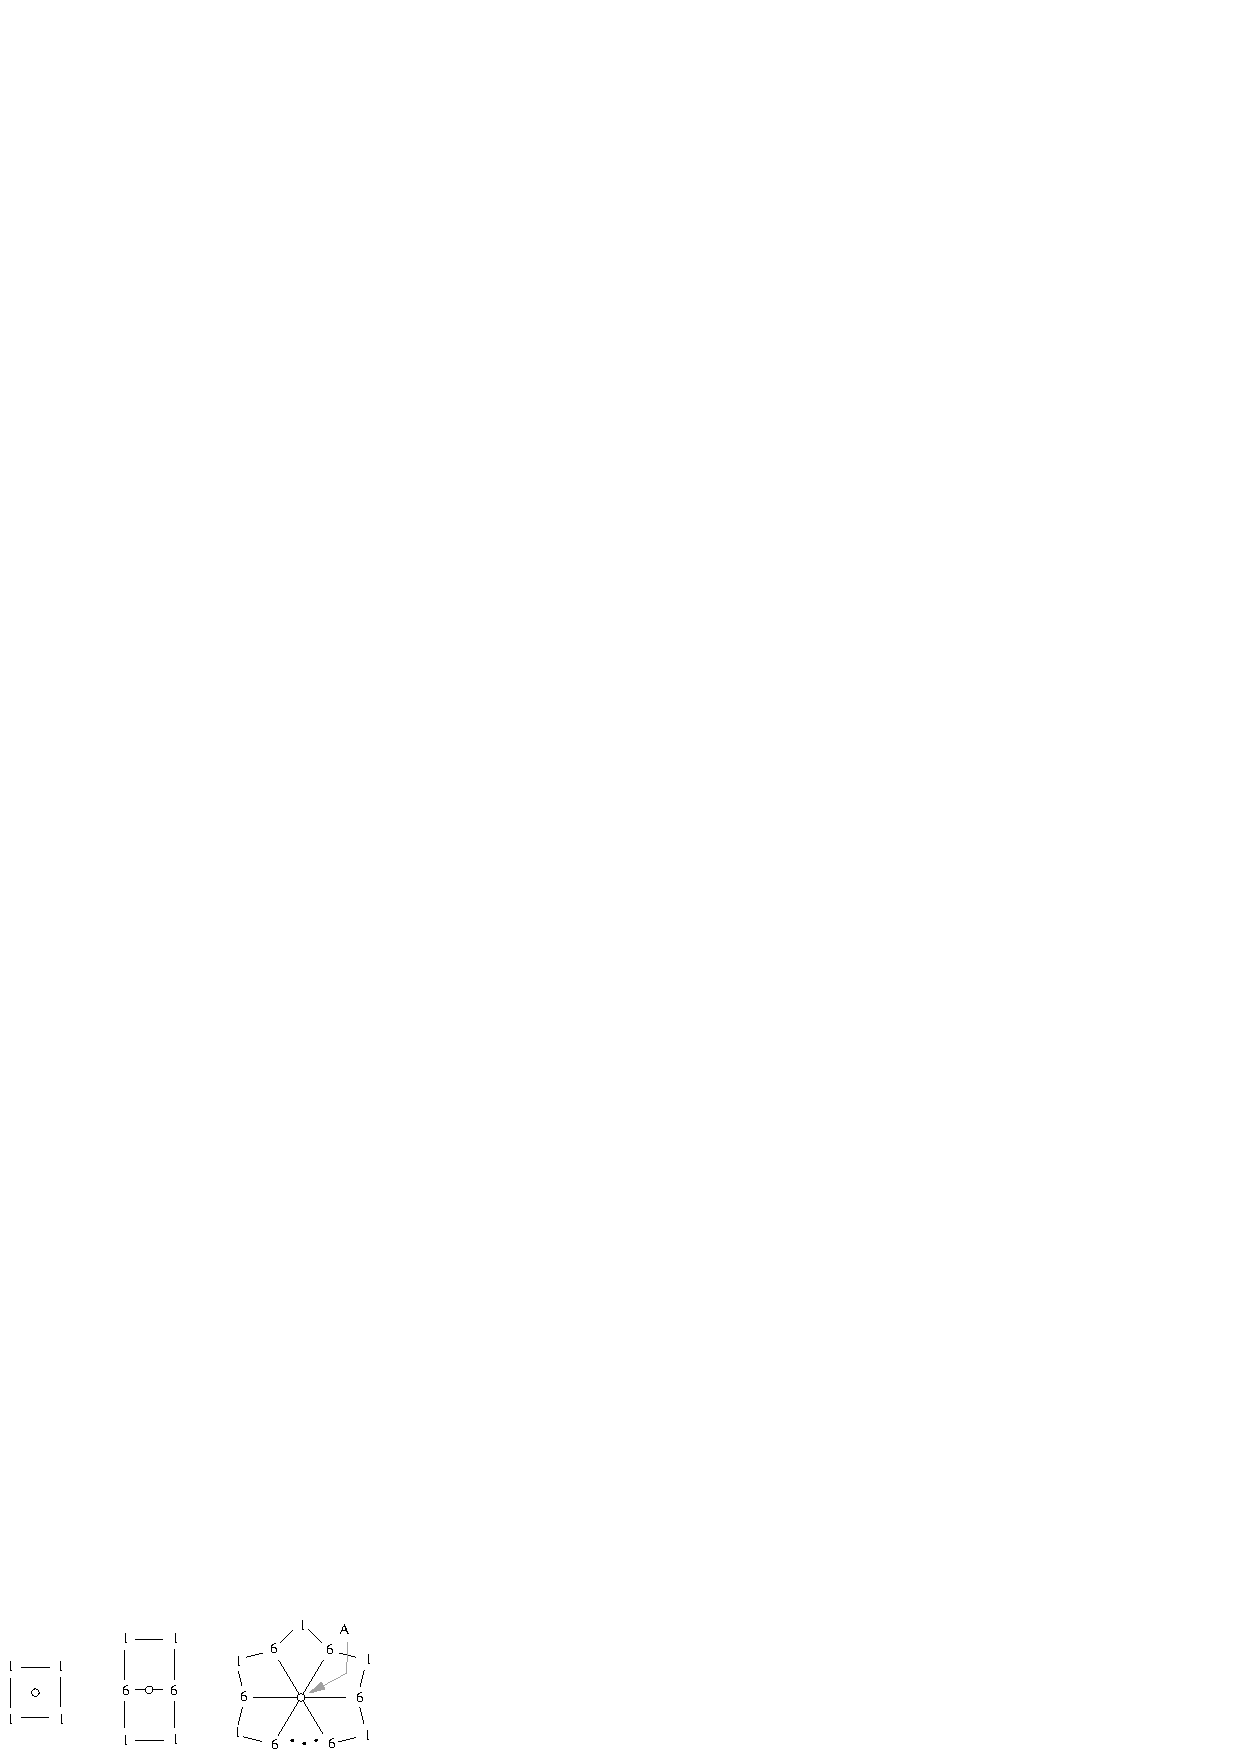
\includegraphics[width=0.4\textwidth]{\FIGDIR/cc_mask}%
%    }
%  \end{center}
%\end{ccTexOnly}

%\begin{ccHtmlOnly}
%  <CENTER>
%  <A HREF="./FIG/cc_mask.gif">
%     <img src="./FIG/cc_mask.gif" alt="Catmull-Clark geometry stencil"></A><P>
%  </CENTER>
%\end{ccHtmlOnly}


% +------------------------------------------------------------------------+
\section{Built-in subdivision schemes}
% +------------------------------------------------------------------------+
Considering their popularity in graphics modeling, 
Catmull-Clark, Loop, \DS\ and $\sqrt{3}$ subdivisions are directly
supported in \ccc{Subdivision_method_3}. 
%Each of these subdivision schemes is realized by parameterizing 
%the corresponding geometry policy to the .

\begin{ccExampleCode}
  static void CatmullClark_subdivision(Polyhedron& p, int step) {
    PQQ(p, CatmullClark_stencil_3<Polyhedron>(), step);
  }
  static void Loop_subdivision(Polyhedron& p, int step) {
    PTQ(p, Loop_stencil_3<Polyhedron>() , step);
  }
  static void DooSabin_subdivision(Polyhedron& p, int step) {
    DQQ(p, DooSabin_stencil_3<Polyhedron>(), step);
  }
  static void Sqrt3_subdivision(Polyhedron& p, int step) {
    Sqrt3(p, Sqrt3_stencil_3<Polyhedron>(), step);
  }
\end{ccExampleCode}

The following shows an example of \DS\ subdivision on a polyhedral mesh.
\ccIncludeExampleCode{Subdivision_method_3/DooSabin_subdivision.C}

% +------------------------------------------------------------------------+
\section{Customize subdivision schemes}
% +------------------------------------------------------------------------+
One of the goals of \ccc{Subdivision_method_3} is 
to provide a flexible platform
to develop user-flavored subdivision schemes.
To construct a customized subdivision scheme, users can simply 
choose a refinement host with the intended topological pattern, 
and then realize the geometry policy accordingly. 
The following example develops a subdivision scheme
generating improved Loop subdivision surfaces. Loop subdivision is
based on PTQ refinement. The geometry policy is developed as a subclass 
of \ccc{PQQ_stencil_3}, which defines the superset of PTQ stencils.

\ccIncludeExampleCode{Subdivision_method_3/Customized_subdivision.C}

A policy function for subdivision surfaces assigns a point on 
the subdivided polyhedron. The points are semantically
required to converge to a smoothed surface of the control mesh.
This is the text-book requirement of a subdivision 
surface (it has to be smooth). Since this is the end of the
class, feel free to throw the text-book away and just try yours. 
Good luck though.

